\section{Chrome Extension for Stack Overflow}
\label{sec:chrome}

In the purpose demonstrating recommending related methods in practice, we build a Chrome extension, {\tool}, for the Stack Overflow query code base and GitHub search code corpus, based on our approach of retrieving common co-occurring code. Figure \ref{fig:chrome} shows a screenshot of using the Chrome extension. The highlighted yellow snippet is the query method from SO, and on the right-hand side we present the ranked list of related code fragments from GitHub. 

The Chrome extension demonstrates a real-life use scenario of getting related methods from GitHub for a SO snippet, thus serves as a proof of our concept of recommending related code fragments beyond similarity.
The use scenario will be: suppose the user is searching on Stack Overflow for the question {\ttt how to unzip a folder in java}. The user locates the highlighted yellow snippet as the correct implementation of the query functionality. They are interested in learning the other methods that can be possibly added to their project along with the {\ttt unzip} method. So the user invokes searching on {\tool} and gets recommended related methods. They may investigate the recommended results and select to add a {\ttt zip} method to complete the functionalities of file manipulation. 

\begin{figure*}[!h]
	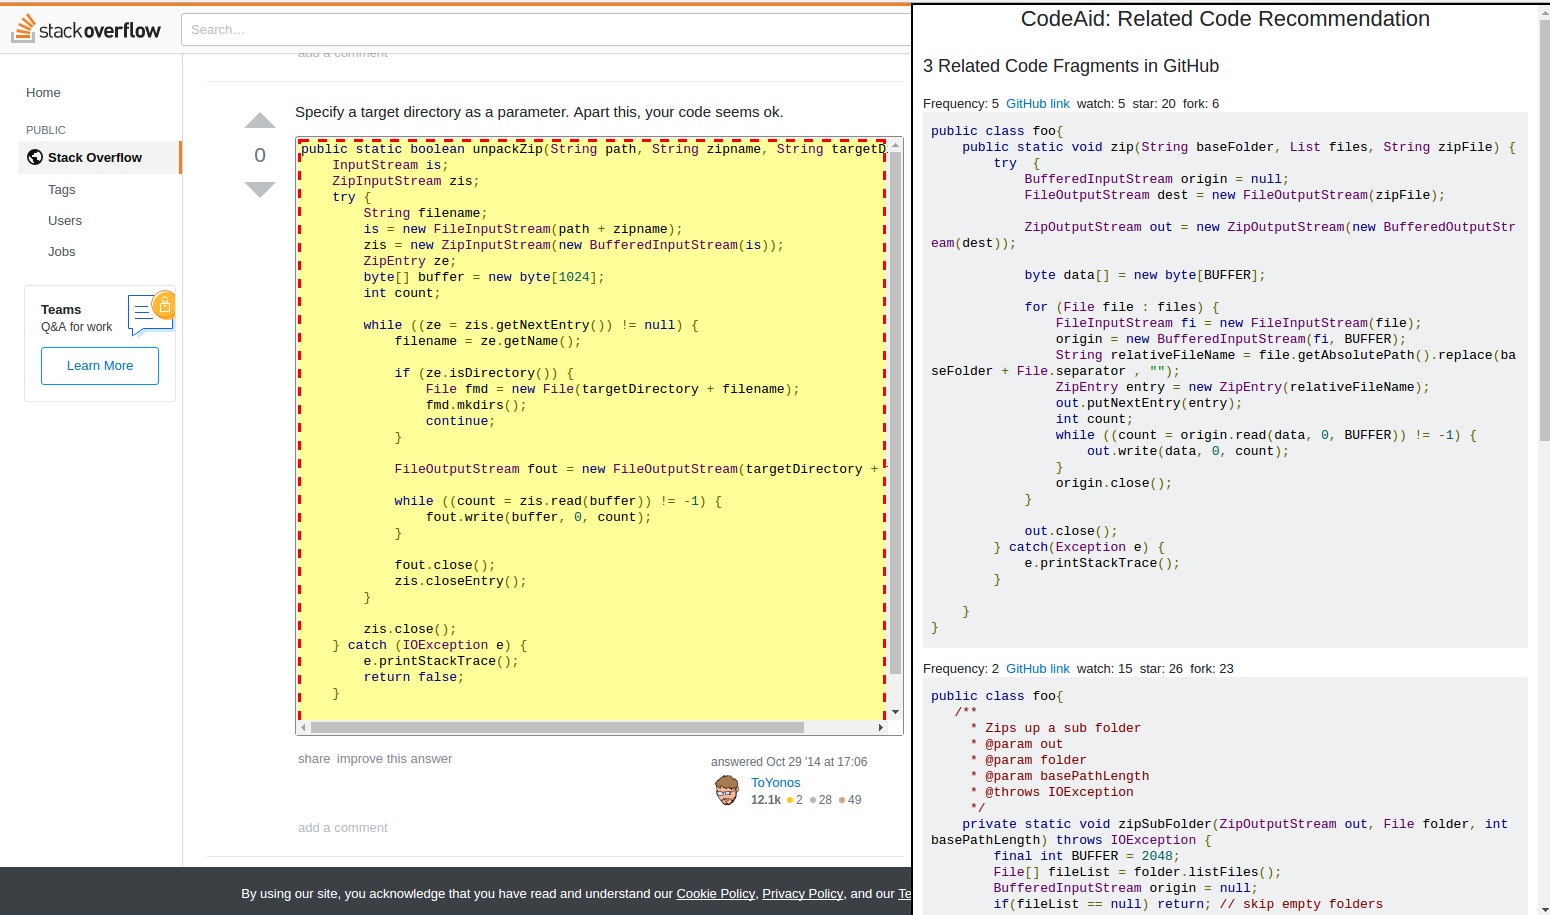
\includegraphics[width=\linewidth]{figures/ui.png}
	\caption{Screenshot of Chrome extension}
	\label{fig:chrome}
\end{figure*}

\subsection{Comparison with code search engines}
In this experiment we compare the recommendation results of \tool\ with those from code search engines. We choose Google search engine since its the most popular destination when people look for programming assistance. We also compare to {\ttt FaCoY}~\cite{kim2018Facoy}, a code-to-code search engine which proved to have state-of-art precision. It uses SO snippets as its query base and indexes GitHub files as search space. {\ttt searchcode}~\cite{searchcode} and {\ttt Krugle}~\cite{krugle} are another two online code-to-code search engines. We only compare with {\ttt FaCoY} because it beats {\ttt searchcode} and {\ttt Krugle} in the total number of outputs and precision of outputs when using SO snippets as queries~\cite{kim2018Facoy}. 
We look for whether the search engines can also retrieve top 1 related code fragments recommended by \tool\ in their top 10 search results. 

For one out of the ten queries, {\ttt FaCoY} can return the related code recommended by \tool\ in its top 10 search results. This results from the related code being very similar to the query, as shown in Table ~\ref{tab:facoy-example}. For the rest of nine queries, the related code is not similar to the query, so it cannot be retrieved by {\ttt FaCoY}.

As for Google search engine, for five out of the ten queries, Google can locate the GitHub file(s) which contain similar methods to the query, therefore we can find the related code recommended by \tool\ inside these GitHub files. However, Google can only retrieve the full files, while \tool\ can point to the method which is mostly used among these files. 

By performing the comparison above, we can see that code search engines may not fulfill the purpose of recommending related code as \tool{}.


\lstset{
	frame=none,
	aboveskip=0pt,
	belowskip=0pt,
	basicstyle=\tiny\ttfamily,
}
\begin{table*}\scriptsize
	\caption{Related code which can be retrieved by FaCoY}
	\label{tab:facoy-example}
	
	\setlength{\tabcolsep}{0.01\textwidth}
	\begin{tabular}{@{}p{0.49\textwidth}p{0.49\textwidth}@{}}
		\toprule
		Query Code Snippet & Recommended Related Code \\
		\midrule


\begin{lstlisting}
public int readFramesChanel(short[] sampleBuffer, int offset, int numFramesToRead,int channel) throws IOException, WavFileException
{
	if (ioState != IOState.READING) throw new IOException("Cannot read from WavFile instance");

	for (int f=0 ; f<numFramesToRead ; f++)
	{
		if (frameCounter == numFrames) return f;

		for (int c=0 ; c<numChannels ; c++)
		{
			if(channel==c)
			{
				sampleBuffer[offset] = (short) readSample();
				offset ++;
			}
			else
				readSample();
		}

		frameCounter ++;
	}

	return numFramesToRead;
}
\end{lstlisting}
		
		&
\begin{lstlisting}
public int writeFrames(int[] sampleBuffer, final int offSetIn, int numFramesToWrite) throws IOException
{
	if (this.ioState != IOState.WRITING) throw new IOException("Cannot write to WavFile instance"); //$NON-NLS-1$
	int offSet = offSetIn;
	for (int f = 0; f < numFramesToWrite; f++)
	{
		if (this.frameCounter == this.numFrames) return f;

		for (int c = 0; c < this.numChannels; c++)
		{
			writeSample(sampleBuffer[offSet]);
			offSet++;
		}

		this.frameCounter++;
	}

	return numFramesToWrite;
}
		
\end{lstlisting}
\\

\bottomrule
	\end{tabular}
\end{table*}
		

